 \documentclass[12pt,fleqn,a4paper]{article}
\linespread{1.3}
\usepackage{tikz}
\usepackage{amsthm,amssymb,amsmath,latexsym,amscd}
\usepackage[top=30mm, bottom=25mm, left=25mm, right=35mm]{geometry}
\usepackage{graphicx}
\usepackage{framed}
\usepackage{mdframed}
\usepackage{lastpage}
\usepackage[pagebackref=false,colorlinks,linkcolor=blue,citecolor=magenta]{hyperref}
\usepackage{fancyhdr}
\usepackage[nottoc]{tocbibind}
\usepackage{xepersian}
\settextfont[Scale=1.1]{Yas}
% چنانچه می‌خواهید اعداد در فرمول‌ها، انگلیسی باشد، خط زیر را غیرفعال کنید
\setdigitfont[Scale=1.1]{Yas}
\pagestyle{empty}
%\newcommand{\Sp}{{\mathcal S}_{\mathcal P}}    
%------------------------------------------------
\begin{document}
%\baselineskip=0.95cm

\begin{center}
{\bf گراف}
\end{center}

\vspace{2cm}
\begin{center}
{\bf سوالات سری اول:}
\end{center}

{\bf 
1- گزینه 3:
}

این تابع زمانی مربوط به الگوریتم مرتب سازی ادغامی است که در این روش برای مرتب سازی $n$ عنصری آنها را به دو زیر آرایه ی 
$\dfrac{n}{2}$ عنصری تقسیم می کنیم و هر دو زیر آرایه را مرتب می کنیم  و در نهایت این دو زیرآرایه با یکدیگر merge  می شوند.

{\bf 
3- گزینه 1:
}

این تابع بصورت بازگشتی، به تعداد $b$ بار، $a$  را در خودش ضرب می کند که معادل است با $a^b$.

{\bf 5- گزینه ی 2:}

\begin{eqnarray*}
F(3,6) 
&=& F(2,6) + F(2,5) \\
&=& F(1,6) + F(1,5) + F(1,5) + F(1,4) \\
&=& 1 + 1 + 1 + 1 \\
&=& 4
\end{eqnarray*}

{\bf 7- گزینه 1:}

برای گره های $E$و  $D$و  $B$ مقدار این تابع برابر با صفر است و برای گره های $C$ و $A$ مقدار این تابع برابر است با مجموع مقدار زیرشاخه های چپ و راست به اضافه ی 1.


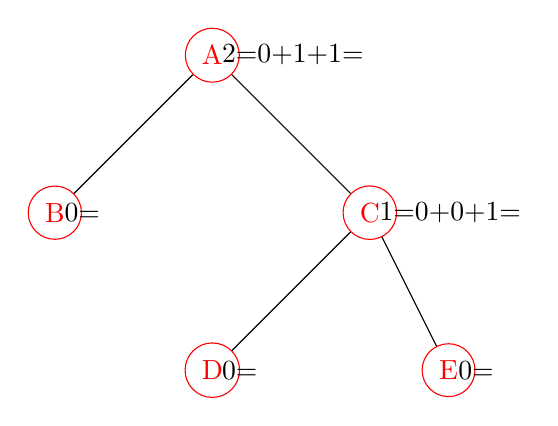
\begin{tikzpicture}
\draw 
(0, 4) node[circle, red, draw](a){A}
(-2, 2) node[circle, red, draw](b){B}
(2, 2) node[circle, red, draw](c){C}
(0, 0) node[circle, red, draw](d){D}
(3, 0) node[circle, red, draw](e){E};

\draw[-] (a) -- node[right] {{2=0+1+1=}} (a);
\draw[-] (b) -- node[right] {0=} (b);
\draw[-] (c) -- node[right] {\ltr{1=0+0+1=}} (c);
\draw[-] (d) -- node[right] {0=} (d);
\draw[-] (e) -- node[right] {0=} (e);
\draw[-] (a) -- (b);
\draw[-] (a) -- (c);
\draw[-] (c) -- (d);
\draw[-] (c) -- (e);
\end{tikzpicture}

{\bf 9- گزینه ی 1:}

\begin{equation*}
T(n)=3T(\frac{n}{4})+\underbrace{n}_{f(n)} 
\stackrel{\text{(master)}\text{قضیه اصلی}}{\Longrightarrow}
n^{\log_b^a}=n^{\log_4^3}	
\end{equation*}

از آنجایی که $f(n)=n>n^{\log_4^3}$ نتیجه می گیریم که مرتبه ی زمانی این تابع برابر با $f(n)$ یا همان $n$ است.

{\bf 11- گزینه 3:}

در روش جستجوی دودویی برای این لیست، ابتدا عنصر وسط این لیست یعنی عدد 23 را با 18 مقایسه می کنیم و چون 18 از کوچکتر است به نیمه ی سمت چپ این لیست می رویم. حال عنصر وسط نیمه ی سمت چپ برابر با عدد 18 است که همان عنصری است که دنبال آن بودیم، یعنی با دو مقایسه به عنصر مورد نظر رسیدیم.

{\bf 13- گزینه ی 2:}

پیچیدگی زمانی الگوریتم مرتب سازی سریع در بدترین حالت برابر با $\Theta(n^2)$ است که مربوط به زمانی است که لیست ورودی از قبل مرتب شده باشد.

{\bf 15-}
در روش کروسکال برای این گراف، ابتدا یال $o1$ و سپس یال 12 و سپس یال 23 که به ترتیب دارای کمترین وزن هستند انتخاب می شوند. لذا گزینه ی 4 صحیح است.

{\bf 17- گزینه ی 3:}

ابتدا ماتریس های $C$ و $B$ که به ترتیب دارای 30 ستون و 30 سطر هستند در یکدیگر ضرب می شوند که حاصل این ضرب، یک ماتریس
$2\times12$
 است. حال این ماتریس در ماتریس $D$ ضرب می شود که حاصل این ضرب، یک ماتریس $2\times8$ است و در نهایت این ماتریس در ماتریس $A$ ضرب می شود تا کمترین تعداد عمل ضرب انجام شود.

{\bf 19- گزینه 3:}

این گزینه اشتباه است زیرا درخت تصمیم در تکنیک عقبگرد نیز کاربرد دارد.

{\bf 21- گزینه ی 3:}

روش انتخاب و تحدید، شکل بهبودیافته ای از روش تقسیم و حل نمی باشد لذا عبارت "ب" اشتباه می باشد و عبارت های "الف" و "ج" در مورد روش انتخاب و تحدید صحیح می باشند لذا گزینه ی 3 صحیح است.

{\bf 23- گزینه ی 2:}

در این گراف فاصله ی بین گره های 2 و 1 برابر با 9 است و همچنین فاصله ی بین گره های 2 و 5 برابر با بی نهایت است زیرا هیچ یال مستقیمی بین این گره وجود ندارد. و این فاصله ها فقط در ماتریس گزینه ی 2 به درستی نوشته شده اند.

{\bf 25- گزینه 3:}

برای مسئله رنگ آمیزی گراف، هیچ الگوریتمی با مرتبه ی زمانی چندجمله ای وجود ندارد و جزو مسائل  Np-Cmplete می باشد. برای سایر گزینه ها، الگوریتم هایی با مرتبه ی زمانی چندجمله ای وجود دارد.

\vspace{2cm}
\begin{center}

{\bf سوالات تشریحی سری اول}
\end{center}
1- از روش حل رابطه ی بازگشتی همگن استفاده می کنیم:
\begin{equation*}
T(n)=
\left\lbrace\begin{array}{c l}3T(n-1)+4T(n-2) ~~~~~\mbox{if}~~~~~ n\geq2,\\t(0)=0, t(1)=1.\end{array}\right.
\end{equation*}

\begin{equation*}
T(n)=3T(n-1)+4T(n-2)\\
\Longrightarrow~~~T(n)-3T(n-1)-4T(n-2)=0\\
\stackrel{\text{مقدار مشخصه}}{\Longrightarrow}
r^2-3r-4=0
\end{equation*}

\begin{equation*}
\Longrightarrow~~~
(r-4)(r+1)=0
\Longrightarrow~~~
\left\lbrace\begin{array}{c l}r_1=4,\\r_2=-1.\end{array}\right.
\Longrightarrow~~~
T(n)=C_12^n+C_2(-1)^n
\end{equation*}

\begin{eqnarray*}
T(0)=0 &\to& C_12^0+C_2(-1)^0 = 0 \to C_1+C_2=0 \\
T(1)=1 &\to& 2C_1-C_2=1 \to 2C_1-C_2=0 \\
&\Longrightarrow&
\left\lbrace\begin{array}{c l}C_1+C_2=0,\\2C_1-C_2=1.\end{array}\right.\\
&\Longrightarrow&
3C_1=1 \to \boxed{C_1=\dfrac13}, \boxed{C_2=-\dfrac13} \\
&\to& \boxed{T(n)=\dfrac132^n-\dfrac13(-1)^n}
\end{eqnarray*}
مرتبه اجرائی این رابطه "نمائی" است.

3- با استفاده از روش حریصانه، کاری را که دارای بیشترین بهره است را انتخاب می کنیم و انجام آن کار را تا آخرین لحظه ی ممکن به تعویق می اندازیم یعنی در این سوال، ابتدا کار شماره 1 که دارای بهره 60 است را برای انجام انتخاب می کنم و انجام آن کار را به  لحظه ی 3 تخصیص می دهیم. حال کار بعدی برای انجام را انتخاب می کنیم که در این مرحله، کار شماره 2 برای لحظه ی 1 انتخاب می شود و در نهایت کار شماره 4 برای لحظه ی 2 انتخاب می شود:

\begin{center}
\begin{tabular}{|c|c|c|c|}
\hline 3 & 2 & 1 & مهلت \\ 
\hline 1 & 4 & 2 & شماره کار \\ 
\hline 60 & 20 & 50 & بهره \\ 
\hline 
\end{tabular}
\end{center}

سود نهایی 
$50+20+60=130$.

5- برای حل این مسئله با روش پویا از تعاریف زیر استفاده می کنیم

مجموعه همه ی رئوس گراف = V

زیرمجموعه ای از رئوس گراف = A

طول کوتاه ترین مسیر از $V_i$  به $V_1$ که از هر راس زیرمجموعه $A$ دقیقا یکبار می گذرد
$ D[V_i][A]=$
در این سوال اگر $A=\{V_3\}$ باشد داریم:

$$D[V_2][A]=len[V_2,V_3,V_1]=\infty$$
ماتریس همجواری این گراف بصورت مقابل است:

\begin{center}
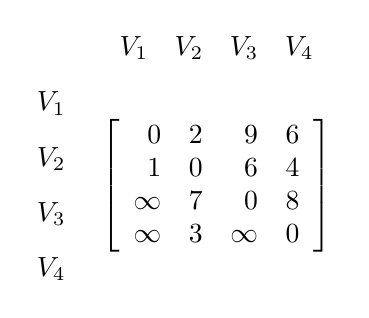
\begin{tikzpicture}[scale=.7]
\node at (0,0) {$\left[\begin{array}{rrrr}
0 & 2 & 9 & 6 \\ 1 & 0 & 6 & 4 \\ \infty & 7 & 0 & 8 \\ \infty & 3 & \infty & 0
\end{array}\right]$};

%	\draw [->] [thin, red] (4.5,-0.7) -- (3.1,-0.7);
%	\node [right, red] at (4.5, -0.7) {$\mbox{مرتبه}$};

\node at (-3,1.5) {$V_1$};
\node at (-3,0.5) {$V_2$};
\node at (-3,-0.5) {$V_3$};
\node at (-3,-1.5) {$V_4$};

\node at (-1.5,2.5) {$V_1$};
\node at (-0.5,2.5) {$V_2$};
\node at (0.5,2.5) {$V_3$};
\node at (1.5,2.5) {$V_4$};
\end{tikzpicture}
\end{center}

و با استفاده از روش برنامه نویسی پویا، قدر بهینه ای که برای این گراف بدست می آید برابر است با:
\[
[V_1, V_3, V_4, V_2, V_1]=21
\]

\vspace{2cm}
\begin{center}

{\bf سوالات سری دوم:}
\end{center}
{\bf 2- گزینه 4:}

در این الگوریتم حلقه ی اول به اندازه ی $n$ بار اجرا می شود ولی تعداد اجرای حلقه دوم وابسته به مجموع عناصر آرایه ی $A$ در اندیس $i$ است، لذا مرتبه ی اجرائی این الگوریتم برابر با $O(n+m)$ است.

{\bf 4- گزینه 3:}

از آنجایی که حاصل $\lim_{n\to\infty}\dfrac{f(n)}{g(n)}$ برابر با یک عدد ثابت شده است می توان نتیجه گرفت که :
$$(f(n)\in\Theta\left(g(n)\right)$$

{\bf 6- گزینه ی 3:}

این رابطه ی بازگشتی را به ازای $f(a,9)$ حل می کنیم:
\begin{eqnarray*}
f(a,9)
&=& a[9] + f(a,7) \\
&=& 10 + 8 + f(a,5) \\
&=& 10 + 8 + 6 + f(a,3) \\
&=& 10 + 8 + 6 + 4 + f(a,1) \\
&=& 10 + 8 + 6 + 4 + 2 + f(a,-1) \\
&=& 10 + 8 + 6 + 4 + 2 + 1 \\
&=& 31
\end{eqnarray*}

{\bf 8- گزینه 4:}
\begin{eqnarray*}
f(n)
&=& f(n-2) * f(n-2) = \left(f(n-2)\right)^2 \to 2^\frac22=2 \\
&=& f(n-4) * f(n-4) * f(n-4) * f(n-4) = \left(f(n-4)\right)^4 \to 2^\frac42=4 \\
&=& f(n-6) * f(n-6) * f(n-6) * f(n-6) *f(n-6) * f(n-6) \\
&& =\left(f(n-6)\right)^8 \to 2^\frac62=8 \\
&\Longrightarrow& f(n)\in o(2^\frac{n}{2})
\end{eqnarray*}

{\bf 10- گزینه 2:}

\begin{tikzpicture}
\draw 
(-3,0) node[circle(1), red, draw](a){1}
(-2,0) node[circle(1), red, draw](b){2}
(-1,0) node[circle(1), red, draw](c){3}
(0,0) node[circle(1), red, draw](d){4}
(1, 0) node[circle(1), red, draw](e){5}
(2, 0) node[circle(1), red, draw](f){6}
(3, 0) node[circle(1), red, draw](g){7}

(-3, -1) node[circle, green, draw](h){3}
(-2, -1) node[circle, green, draw](i){2}
(0, -1) node[circle, green, draw](j){1};

\draw [->] [thick, blue] (-3,-0.7) -- (-3,-0.3);
\draw [->] [thick, blue] (-2,-0.7) -- (-2,-0.3);
\draw [->] [thick, blue] (0,-0.7) -- (0,-0.3);
%\draw[-] (e) -- node[right] {0=} (e);
%\draw[-] (a) -- (b);
\end{tikzpicture}

در یک آرایه ی 7 عنصری مطابق آرایه ی مقابل ابتدا عنصر مورد نظر با عنصر میانی آرایه مقایسه می شود و اگر کوچکتر از عنصر میانی بود به سمت چپ آرایه می رویم و با عنصر میانی زیرآرایه ی چپ مقایسه می کنم و اگر برابر نبوده باز به زیرآرایه ی سمت چپ می رویم که در مجموع برابر با 3 مقایسه می شود. 
برای حالتی که عنصر موردنظر از عنصر میانی بزرگتر باشد به زیرآرایه سمت راست می رویم که باز هم نیاز به 3 مقایسه است و در حالت متوسط به 3 مقایسه در جستجوی ناموفق نیاز داریم.

{\bf 13- گزینه ی3:}

تعداد عمل ضرب در روش پویا برابر با $n^3$ می باشد که این مقدار برای ضرب ماتریس های $8\times8$ برابر با $8^3=512$ عمل ضرب می باشد. در ضرب ماتریس ها به روش استراسن در مرحله ی اول نیاز به 343 ضرب و در مرحله نهایی نیاز به 49 ضرب است که در مجموع برابر با 392 ضرب می باشد.

{\bf 14- گزینه 3:}

با استفاده از روش هار حریصانه اگر بصورت جدول زیر کارها را انجام بدهیم، سود بدست آمده برابر با 121 می شود که این میزان سود برابر با بیشترین سود ممکن برای این مسئله است:

\begin{center}
\begin{tabular}{|c|c|c|c|c|c|c|c|}
\hline \rule[-1ex]{0pt}{2.5ex} 11 & 2 & 6 & 10 & 3 & 7 & 1 & شماره کار \\ 
\hline \rule[-1ex]{0pt}{2.5ex} 7 & 6 & 5 & 4 & 3 & 2 & 1 & بازه زمانی \\ 
\hline \rule[-1ex]{0pt}{2.5ex} 4 & 7 & 16 & 23 & 25 & 27 & 19 & سود \\ 
\hline 
\end{tabular}
\end{center}

{\bf 16- گزینه 1:}

این الگوریتم بیانگر رابطه ی محاسبه ی ضریب دوجمله ای است که به صورت زیر بیان می شود:

$$\binom{n}{k}=\binom{n-1}{k-1}+\binom{n-1}{k}$$
که این رابطه نیاز به 
$\binom{n}{k}-1$ 
عمل جمع دارد.

{\bf 18- گزینه ی 3:}

حداکثر تعداد بازی زمانی اتفاق می افتد که تیم های $A$ و $B$ به ترتیب برنده شوند. به عنوان مثال در بازی اول، تیم $A$ برنده شود و در بازی دوم تیم $B$  برنده شود و در بازی سوم تیم $A$ و در بازی چهارم تیم $B$ برنده شوند و این روال ادامه پیدا کند. در این صورت حداکثر بازی مورد نیاز برابر با $2n-1$ می باشد.

{\bf 20- گزینه 2:}

می خواهیم تعداد درخت های جستجوی دودویی متفاوت با $n$ کلید متمایز را بدست آوریم. فرض کنید که گره های هر کدام از این درخت ها را به روش میان ترتیب از 1 تا $n$ شماره گذاری می کنیم. با این شماره گذاری فرض کنید که شماره $1\leqslant i\leqslant n$ ریشه درخت باشد. در آن صورت زیر درخت راست آن حتما باید $n-i$ گره داشته باشد. 

حال اگر $T(n)$  تعداد درخت دودویی با $n$ گره باشد، تعداد زیردرخت های چپ و راست ریشه به ترتیب برابر با $T(i-1)$ و $T(n-i)$ خواهند بود. در آن صورت اگر گره $i$ ریشه باشد، حاصلضرب $T(i)T(n-i)$ برابر تعداد کل درخت هاست و با در نظر گرفتن همه ی حالات، رابطه ی بازگشتی زیر بدست می آید که همان عدد کاتالان است:
$$\dfrac{1}{n+1}\binom{2n}{n}$$

{\bf 22- گزینه 3:}

روش عقبگرد به طور عمده در مسائل تصمیم گیری استفاده می شود، لذا گزینه ی 3 صحیح است.

{\bf 24- گزینه 2:}

تعداد کل گره های درخت ؟؟؟ حالت برای الگوریتم یافتن مدارهای همیلتونی با استفاده از تکنیک عقبگرد، با استفاده از رابطه ی 
$1+(n-1)+(n-1)^2+\cdots+(n-1)^{n-1}$ 
بدست می آید که این عبارت معادل است با:
$$1+(n-1)+(n-1)^2+\cdots+(n-1)^{n-1}=\dfrac{(n-1)^n-1}{n-2}$$

\vspace{2cm}
\begin{center}

{\bf سوالات تشریحی سری دوم:}
\end{center}
از الگوریتم پریم برای حل این مسئله استفاده می کنیم: ابتدا از گره 1 شروع می کنیم و از بین گره های 2و 3 و 4 که همگی دارای فاصله ی 5 تا گره 1 هستند، یکی را بصورت دلخواه انتخاب می کنیم. در اینجا ما گره شماره 2 را انتخاب می کنیم و طول مورد نیاز تا این مرحله برابر با 5 است. حال گره ای که کمترین فاصله تا مجموعه گره های 
$\{1,2\}$ 
دارد را انتخاب می کنیم که گره ی شماره 3 است و این گره را به این مجموعه اضافه می کنیم:
$\{1,2,3\}$. 
تا به اینجا طول نوار مسی مورد نیاز برابر با 10 است. حال گره ای که کمترین فاصله تا مجموعه ی 
$\{1,2,3\}$ 
دارد را انتخاب می کنیم که گره ی شماره 4 است که دارای فاصله 5 از گره شماره 1 است و این گره به این مجموعه اضافه می شود:
$\{1,2,3,4\}$ 
و طول مورد نیاز نیز در مجموع برابر با 15 می شود. در نهایت گره  شماره 5 که دارای فاصله ی 5 با گره شماره 4 است به این مجموعه
اضافه می شود:
$\{1,2,3,4,5\}$ 
و طول نهایی نوار مسی برابر با  $15+5=20$ می شود.

4- در این روش ابتدا تمامی آیتم ها را بر اساس  $\dfrac{p_i}{w_i}$ مرتب می کنیم:

\begin{center}
\begin{tabular}{|c|c|c|c|}
\hline \rule[-1ex]{0pt}{2.5ex} $\dfrac{p_i}{w_i}$ & $w_i$ & $p_i$ & $i$ \\ 
\hline \rule[-1ex]{0pt}{2.5ex} $1.33$ & 15 & 20 & 5 \\ 
\hline \rule[-1ex]{0pt}{2.5ex} $1.25$ & 8 & 10 & 2 \\ 
\hline \rule[-1ex]{0pt}{2.5ex} $0.6$ & 25 & 15 & 4 \\ 
\hline \rule[-1ex]{0pt}{2.5ex} $0.5$ & 16 & 8 & 1 \\ 
\hline \rule[-1ex]{0pt}{2.5ex} $0.33$ & 15 & 5 & 3 \\ 
\hline 
\end{tabular}
\end{center}

در ابتدا کوله پشتی خالی است و وزن و ارزش قطعات برابر با صفر است:
\begin{equation*}
	\left\lbrace\begin{array}{c l}w=0,\\p=0.\end{array}\right.
\end{equation*}

حال مطابق درخت زیر، قطعه شماره 5 را به کوله پشتی اضافه می کنیم
\begin{equation*}
	\left\lbrace\begin{array}{c l}w=15,\\p=20.\end{array}\right.
\end{equation*}
در مرحله بعد گره شماره 2 به این درخت اضافه می شود

\begin{equation*}
	\left\lbrace\begin{array}{c l}w=15+8=23,\\p=20+10=30.\end{array}\right.
\end{equation*}

حال اگر آیتم های 3 یا 4 به درخت اضافه شوند، وزن مجموع، از وزن مجاز بیشتر می شوند، در نتیجه این گره ها انتخاب نمی شوند و به آیتم 2 برمی گردیم و آیتم شماره 1 انتخاب می شود

\begin{equation*}
	\left\lbrace\begin{array}{c l}w=39,\\p=38.\end{array}\right.
\end{equation*}

حال اگر گره های 3 یا 4 را به این درخت اضافه کنیم، وزن مجموع از حد مجاز خارج می شود، در نتیجه عقبگرد می کنیم و به آیتم 5 بر می گردیم. حال می توانیم گره 4 را اضافه کنیم و ادامه بدهیم ولی همانطور که در درخت زیر مشاهده می کنیم، بیشترین سود بدست آمده برابر با 38 و وزن قطعات برابر با 39 می شود:

\begin{center}
\begin{tikzpicture}
\draw 
(0, 6) node[circle, red, draw](a){\tiny{\begin{matrix}w=15,\\p=20 \end{matrix}}}
(-2, 4) node[circle, red, draw](b){\tiny{\begin{matrix}w=23,\\p=30 \end{matrix}}}
(2, 4) node[circle, red, draw](c){\tiny{\begin{matrix}w=40,\\p=35 \end{matrix}}}
(0.8, 1) node[circle, red, draw](d){w=48}
(2.4, 1) node[circle, red, draw](e){w=56}
(4, 1) node[circle, red, draw](f){w=55}
(-0.8, 1) node[circle, red, draw](i){\color{green}{\tiny{\begin{matrix}w=39,\\p=38 \end{matrix}}}}
(-2.4, 1) node[circle, red, draw](h){w=48}
(-4, 1) node[circle, red, draw](g){w=48}
(-0.5, -2) node[circle, red, draw](m){w=64}
(1.5, -2) node[circle, red, draw](n){w=54};

\draw[-] (a) -- node[above] {5} (a);
\draw[-] (b) -- node[above] {2} (b);
\draw[-] (c) -- node[above] {4} (c);
\draw[-] (d) -- node[above] {2} (d);
\draw[-] (e) -- node[above] {1} (e);
\draw[-] (f) -- node[above] {3} (f);
\draw[-] (g) -- node[above] {3} (g);
\draw[-] (h) -- node[above] {4} (h);
\draw[-] (i) -- node[above] {1} (i);
\draw[-] (m) -- node[above] {3} (m);
\draw[-] (n) -- node[above] {4} (n);

\draw[-] (a) -- (b);
\draw[-] (a) -- (c);
\draw[-] (c) -- (d);
\draw[-] (c) -- (e);
\draw[-] (c) -- (f);
\draw[-] (b) -- (g);
\draw[-] (b) -- (h);
\draw[-] (b) -- (i);
\draw[-] (d) -- (m);
\draw[-] (d) -- (n);
\end{tikzpicture}
\end{center}



\end{document}


بجای merge می تونی بنویسی ادغام
توی سوال 11 خط دوم یه چیزی از قلم افتاده
